\section{Grundlagen}
\label{sec:grundlagen}

Folgendes Kapitel beschreibt die Robotik und die benötige Einordnung der Arbeit in diese.
Hierfür wird die Robotik oberflächlich definiert, eingeteilt und die relevanten Teilbereiche dieser genauer betrachtet.
Da diese Arbeit sich mit einem \gls{go1} beschäftigt, wird dieser klassifiziert und in die Bereiche der Forschung, Industrie und weiterer Nutzung eingeordnet.
Zum weiteren Verständnis des Ziels der Arbeit - der Analyse und Integration des \gls{go1} in ein bestehendes Ökosystem -
wird der aktuelle Stand der Forschung genauer betrachtet.
Relevant sind hier besonders die bereits erarbeiteten Erkenntnisse der Nutzung gleicher oder ähnlicher Roboter, als auch
die Einbindung anderer Modelle in bestehende Ökosysteme.
Hierfür soll nicht nur die Forschung allein betrachtet werden, sondern auch die Arbeit privater Unternehmen und Entwickler.
Mit dem Wissen der korrekten Einordnung des \gls{go1} und dem Forschungsstand zu verwandten Themen sollen die Herausforderungen dieser
Arbeit hervorgehoben werden, sodass im späteren Verlauf die Erarbeitungen auf die bekannten Probleme verweisen können.

\subsection{Robotik}
\label{subsec:robotik}

Die Robotik befasst sich mit dem Wissensgebiet rund um \emph{Roboter}.
Der Begriff \emph{Roboter} stammt vom tschechischen Wort \emph{robota}, was so viel wie \emph{Frondienst} oder \emph{Zwangsdienst} bedeutet.
So treffend diese Übersetzung auf die heutige Nutzung des Wortes ist, so vage ist diese Beschreibung auch.
Ähnlich unklar sind auch die anerkannten Definitionen des Wortes \emph{Roboter}.
Eine gängige Definition im deutschsprachigen Raum ist die des \gls{vdi}:

\begin{quote}
    Industrieroboter sind universell einsetzbare Bewegungsautomaten mit mehreren Achsen,
    deren Bewegungen hinsichtlich Bewegungsfolge und Wegen bzw.
    Winkeln frei (d.h, ohne mechanischen Eingriff) programmierbar und ggf.~sensorgeführt sind\footcite{vdi_2860}.
\end{quote}

Auch wenn die \gls{vdi}-Richtlinie mittlerweile zurückgezogen wurde, wird die Definition aufgrund ihrer treffenden Eingrenzung
des Begriffes noch häufig zitiert.

Die umstrittene Definition des Begriffs \emph{Roboter} zieht eine ebenso unklare Einteilung des Wissensfeldes der \emph{Robotik} mit sich.
Hält man sich jedoch an die Definition des \gls{vdi}, so lassen sich Roboter in zwei Kategorien einteilen, Industrieroboter und Serviceroboter.
Abbildung~\ref{fig:industrie_vs_service}\footcite{statista_robotics_market} zeigt die beiden Klassifizierungen und deren Eigenschaften im Überblick.

\begin{figure}[h]
    \frame{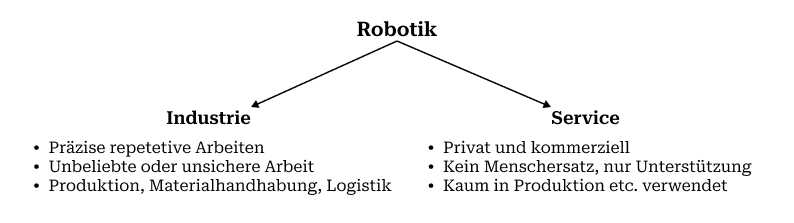
\includegraphics[width=\linewidth]{img/grundlagen/industrie_vs_service}}
    \caption{Vergleich zwischen Industrie- und Servicerobotern}\label{fig:industrie_vs_service}
\end{figure}

\subsubsection{Industrieroboter}

Industrieroboter sind Roboter, die im industriellen Umfeld eingesetzt werden den Mensch meist in nicht sicheren,
nicht rentablen oder nicht begehrenswerten - repetitiven - Arbeiten ersetzen.
Sie sind aufgrund ihrer hohen Spezialisierung an den Einsatzzweck großenteils stationär.
Der Vorteil industriell eingesetzter Roboter ist die hohe Effizienz und Genauigkeit der Arbeiten und die Anpassbarkeit an
den Einsatzzweck.
Als Nachteil ergibt sich hieraus der hohe Aufwand der Implementierung, da ein hoch spezialisierter Roboter für jeden
Einsatzzweck neu geschaffen werden muss.
Einsatzzwecke von Industrierobotern sind unter anderen das Schweißen, Lackieren, Montieren und die Materialhandhabung in
Produktionsumgebungen.

Die Limitierung des Einsatzes und die strikte Einteilung zu industriellen Einsätzen lässt schlussfolgern, dass der \gls{go1}
nicht in die Klasse der Industrieroboter eingegliedert werden kann.
Stattdessen kann man ihn in der in dieser Arbeit verwendeten, einfachen Unterteilung den Servicerobotern zuteilen.

\subsubsection{Serviceroboter}

Serviceroboter unterscheiden sich im Kern von Industrierobotern in der Annahme, dass sie Menschen in ihrem Einsatzzweck nicht ersetzen,
sondern unterstützen oder von Menschen unterstützt werden.
Der Begriff \emph{Serviceroboter} ist absichtlich weit gefasst und schließt im Umfang dieser Arbeit lediglich industrielle
Roboter, so wie sie im vorigen Paragrafen beschrieben werden, aus.
Bei Serviceroboter lässt sich grundsätzlich noch zwischen kommerziell eingesetzten und konsumorientierten Robotern unterscheiden\footcite{statista_robotics_market}.

Serviceroboter sind in der Regel nicht stationär, da sie in ihren Einsatzmöglichkeiten deutlich flexibler sind, als Industrieroboter.
Aus dem Vorteil der Flexibilität lässt sich ebenfalls der Nachteil der Komplexität ableiten.
Das weitere Einsatzfeld der Serviceroboter steigert in der Regel den Aufwand der Entwicklung, steigert aber ebenfalls
den Ertrag des Roboters, finanziell auch den \gls{roi}.

Möchte man die Klasse der Serviceroboter weiter untergliedern, so sind unter anderen folgende Untergliederungen denkbar:

\begin{itemize}
    \item Spielzeugroboter
    \item Erkundungsroboter
    \item Militär-/ Kampfroboter
    \item Assistenzroboter
\end{itemize}

Zu Vermerken ist, dass die simple Klassifizierung der Roboter in lediglich zwei Klassen der Industrieroboter und der Serviceroboter
gewählt wurde, um die Einsatzzwecke des \gls{go1} in dieser Arbeit nicht einzuschränken.
Wie bereits erarbeitet kann man den \gls{go1} vielseitig einsetzen, jedoch ist er nicht geeignet, Menschen in seinen Einsatzgebieten
vollständig zu ersetzen, noch ist er strikt auf industrielle Zwecke beschränkt.
Eine Zuteilung zu industriellen Robotern ist somit nicht möglich.
Eine genauere Klassifizierung innerhalb der Klasse der Serviceroboter ist zwar möglich, jedoch vom finalen Einsatzzweck des
Quadruped Roboters abhängig.
Mögliche Einsatzzwecke werden später in dieser Arbeit erörtert.

\subsubsection{Cobots}

Ein weiterer passender Begriff, der der Klassifizierung des \gls{go1} als Serviceroboter nicht widerspricht, ist \emph{Cobot}
\emph{Cobot} setzt sich aus dem Englischen Wort \emph{collaborate} - (zusammenarbeiten, kollaborieren) und dem Wort \emph{Roboter}
zusammen.
Einige Merkmale sind:\footcite{statista_robotics_market}

\begin{itemize}
    \item Kollaborativ und sicher, im Gegensatz zu stationär und abgesichert
    \item Interaktiv und adaptiv zur Umgebung
    \item Einfache Inbetriebnahme durch vorausschauende Entwicklung
    \item Flexible Einsatzzwecke
    \item Schnelleres \gls{roi}
\end{itemize}

Durch seine flexiblen Fortbewegungsmöglichkeiten und der hohen Anzahl an Sensorik und Erweiterungsmöglichkeiten des \gls{go1}
sowie der zur Kollaboration einladenden Vorrichtungen wie den Mikrofonen und Lautsprechern\footnote{Siehe Kapitel~\ref{subsubsec:sensorik}}
lässt sich der \gls{go1} neben der Klassifizierung als Serviceroboter ebenfalls als \emph{Cobot} bezeichnen.
Der kollaborative Aspekt und die Unterstützung des Menschen statt der Ersetzung dessen wird im Laufe der Arbeit weiter erörtert.
\todo{Herleitung Quadruped}

\subsection{Stand der Forschung}
\label{subsec:stand-der-forschung}

Im Bereich der Quadruped Roboter ist bereits viel erforscht worden.
Besonders im Fokus der Arbeiten sind in der Regel die Steuerung der Motoren zur Fortbewegung, die autonome Navigation
der Roboter in unbekanntem Umfeld und das Testen der Einsatzmöglichkeiten der vierbeinigen Roboter.
Diese Arbeit hingegen beschäftigt sich mit der Integration des Roboters in ein Hochschulökosystem, welche die möglichen Einsatzzwecke
nicht vorwegnimmt.
Ziel dieser Arbeit ist es, Einsatzmöglichkeiten zu erarbeiten und die nötigen Anpassungen am Model \gls{go1} vorzunehmen,
um diese zu ermöglichen.
Deshalb werden im folgenden nur kurz allgemein interessante Forschungen an Quadruped Robotern gezeigt, wonach
allgemeine Forschungen zur Einbindung und Nutzung von Servicerobotern dargestellt werden.
Zuletzt sollen noch Arbeiten speziell zum Modell \gls{go1} gezeigt werden.
Diese werden nicht zwingend akademischen Ursprungs sein und sollen dem Leser der Arbeit einen Überblick über die vorhandenen
Ressourcen zum Modell \gls{go1} bieten.

\subsubsection{Quadruped Roboter}
\label{subsubsec:quadruped-roboter}
% Big Dog
Die erste Umsetzung eines Quadruped Roboters, die öffentliche Aufmerksamkeit erlangte, ist der sogenannte \emph{Big Dog}
der Firma \emph{Boston Dynamics} aus Boston, \gls{usa}.
Dieser wurde \num{2008} aus militärischem Interesse an einer geländegängigen Alternative zu gängigen Militärfahrzeugen entwickelt und
deshalb auch vom amerikanischen \gls{darpa} finanziert. \emph{Big Dog} wurde mit hydraulischen Extremitäten entwickelt, welche ihm ermöglichen sollten,
schweres Gepäck im Militäreinsatz tragen zu können.
Die Flexibilität der vier Beine und die Möglichkeit dieser, sich relativ schnell durch schweres Gelände bewegen zu können,
gaben \emph{Big Dog} einen möglichen Vorteil gegenüber gängigen Fortbewegungsmitteln auf Basis von Ketten oder Rädern.
Weitere Entwicklungen am \emph{Big Dog} wurden später vom \gls{rcta} des \gls{us} Army Research Laboratory finanziert.
\footcite{bigdog}\footcite{darpa_bigdog}

% MIT Cheetah
\num{2009} hat das \emph{Biometric Robotics Lab} des \gls{mit} das Projekt namens \emph{Cheetah} - auf Deutsch \emph{Gepard} -
bekannt gegeben.
Das Projektziel war es, einen Quadruped Roboter zu entwickeln, der in den Bereichen Tempo und Energieeffizienz der echten
Tierwelt Konkurrenz macht.
Auch dieses Projekt wurde vom \gls{darpa} finanziert\footcite{bi_mit_cheetah_funding}\footcite{darpa_m3}.
Im Gegenzug zum \emph{Big Dog} wurde der \emph{Cheetah} aber nie kommerziell oder militärisch beworben.
Stattdessen liegt der Fokus des Roboters im Bereich der Forschung.
Bereits \num{2012} veröffentlichte das \emph{Biometric Robotics Lab} die ersten Videos des Roboters im Lauf.
Seit der Projektankündigung wurden mehrere Iterationen des Roboters entwickelt.
Die aktuelle Iteration des Roboters ist in ihrer Bauart optimiert und somit kostentechnisch effizient im Einkauf und in der Reparatur.
Im Gegensatz zum \emph{Big Dog} ist der \gls{mit} \emph{Cheetah} voll elektrisch, was das Ziel der einfachen Entwicklung hat.
\footcite{ieee_spectrum_cheetah}
Viele Erkenntnisse aus dem \gls{mit} \emph{Cheetah} Projekt werden heute noch in neuen Projekten verwendet.
So auch bei der Umsetzung des \gls{go1}, worauf in dieser Arbeit aber weniger eingegangen wird.
\todo{Akademische forschung als fokus}

% Spot
Die aktuell vermutlich bekannteste Umsetzung eines Quadruped Roboters ist der von \emph{Boston Dynamics} entwickelte
\emph{Spot}, welcher in seiner ersten Form bereits \num{2015} öffentlich beworben wurde.
Anders als seine Vorgänger Roboter bei \emph{Boston Dynamics} war er der erste Roboter der Firma, der zu \num{100}\%
elektrisch betrieben wurde.
Das lässt ihn sehr ähnlich zum \emph{Cheetah} des \gls{mit} wirken, jedoch hatte die Plattform \emph{Spot} von Anfang an den
Fokus auf einen kommerziellen oder auch militärischen Einsatz.
Besonders nennenswert an dem Roboter ist die Kompaktheit seinen Vorgängern gegenüber.
Die aktuelle Version des \emph{Spot} ist bereits kommerziell verfügbar und wurde initial für etwa \num{75000} \gls{us}-Dollar\footcite{spot_price}
zum Kauf beworben.
\footcite{boston_dynamics_legacy}

Die Veranschaulichung \citetitle{quadruped_timeline} gibt einen Überblick über die Zeitschiene der einflussreichsten
Implementierungen von Quadruped Robotern in der jüngeren Vergangenheit\footcite{quadruped_timeline}.
\todo{Bilder der Roboter}

\subsubsection{Integration von Robotern}

Im Bereich der Robotik liegt neben dem Fokus des Testens der Möglichkeiten immer die Suche nach einer sinnvollen Nutzung
der gewonnenen Erkenntnisse und der entwickelten Roboter in realen Szenarien.
Hierbei sind die Möglichkeiten kaum limitiert und hängen stets von der Form und Reife der Roboterimplementierungen ab.
Im Folgenden werden einige aktuelle Ansätze zur Integration und Nutzung von Quadruped Robotern in realen Szenarien vorgestellt.

Die unten genannten Einsatzmöglichkeiten von Quadruped Robotern sind lediglich eine Auswahl des offensichtlichen
Potenzials und sollen lediglich einen Überblick schaffen.
Eine vollständige Auflistung der Integrationsansätze ist hier nicht angestrebt.

% Monitoring
\myparagraph{Kontrolle und Überwachung}
% Construction Monitoring Paper ##
Quadruped Roboter sind aufgrund ihrer Fähigkeit, sich in unstrukturierten Umgebungen fortzubewegen, gut dafür geeignet,
in gefährlicheren Gebieten die Kontrollfunktion des Menschen zu übernehmen.
Zudem kann ein weit genug entwickelter Roboter autonom Aufgaben übernehmen und diese in regelmäßigen Intervallen durchführen,
was einen großen Vorteil dem Menschen gegenüber darstellt.
Eine mögliche Einsatzmöglichkeit von Quadruped Robotern ist laut des Artikels \citetitle{construction_quadruped} das Überwachen und
Prüfen des Fortschritts auf Baustellen.
Die Autoren bezeichnen die manuelle Kontrolle einer Baustelle durch einen menschlichen Inspektor als zeitlich inneffizient,
unstrukturiert und unzuverlässig.
Sie bemängeln zudem, dass die menschlichen Kontrollen aufgrund kleinster Abweichungen in der Systematik kaum wiederholbar sind
und somit schlecht einzuordnen sind.
Ihr Ansatz, die zu kontrollierenden Umgebung zu virtualisieren und dann anhand automatisierter Abläufe und Scans durch
Quadruped Roboter mit den zu erzielenden Ergebnissen abzugleichen birgt zwar einige Hürden, verspricht jedoch
ein konsistentes Ergebnis über den zeitlichen Verlauf der Baustelle hinweg.
Zudem heben die Autoren die zeitliche Ersparnis und somit die Effizienz des Ansatzes hervor, da selbst bei einer nur teilweise
automatisierten Umsetzung ein verteiltes Monitoring möglich ist, bei dem sich nur der Roboter mit Sensorik und Kameras vor Ort befinden muss.
\footcite{construction_quadruped}

Im Bereich der Integration eines solchen Quadruped Roboters im Hochschulumfeld lässt sich dieser Ansatz beispielsweise
in der automatisierten Modellierung des Campus übersetzen.
Ein vorheriges Erstellen eines exakten Modells ist bei diesem Ansatz nicht nötig, man macht sich hier lediglich die 
Möglichkeit der Modellierung durch Sensorik wie beispielsweise Ultraschall, \gls{lidar} und Kameras zu nutzen.


\myparagraph{Sicherheit}
% Public Safety Paper Boston Dynamics ##
Da die Umgebung in urbanen Umgebungen zu großen Teilen unstrukturiert ist, is der Einsatz dedizierter Roboter für den
Betrieb auf Straßen oder in der Luft oft erheblich eingeschränkt.
Neben der flexibleren Manövrierbarkeit von Quadruped Robotern ist die Erweiterbarkeit
dieser ein weiterer Vorteil gegenüber einfacheren Robotern auf Basis von Rädern oder Dronen.
So ermöglicht die Erweiterung eines serienmäßigen \emph{Spot} Roboters durch einen Arm mit Greifer laut der Studie
\citetitle{boston_dynamics_safety} die Gefahrenminimierung für Menschen in Einsatzzwecken wie der Kontrolle verdächtiger Objekte und dem
möglichen Entfernen dieser aus einer Gefahrenzone, dem Aufspüren potenziell gefährlicher Substanzen in der Umgebung (Strahlung, Leckagen, Flüssigkeiten)
oder der vorzeitigen Prüfung einer Umgebung, um den Einsatzkräften in Notfallsituationen einen besseren Überblick zu verschaffen,
ohne sich selbst in Gefahr zu bringen.
\emph{Boston Dynamics} heben in ihrer Studie besonders die hohe Modularität von Quadruped Robotern hervor, welche sie
flexibel einsatzbar macht.
\footcite{boston_dynamics_safety}

Im Umfang dieser Arbeit wäre im Sinne der Sicherheit eine Nutzung des Roboters bei Brandbildung zur Suche nach Verletzten denkbar.
Auch ein Ablaufen der potenziell gefährlichen Labore und der Prüfung nach Leckagen ist denkbar.
Zu Schließzeiten könnten Quadruped Roboter wie der \gls{go1} ebenso genutzt werden, um den Campus nach nicht autorisierten
Besuchern abzusuchen.

\myparagraph{Automatisierung und Effizienz}
Wie in Kapitel \ref{subsec:robotik} erläutert, bringt die Herkunft des Wortes \emph{Roboter} eine der Kernziele der Robotik zum Vorschein.
Die Automatisierung und Entlastung des Menschen bei einfachen oder wenig begehrenswerten Aufgaben liegt hier im Fokus.
So können Roboter einfache und repetitive Aufgaben übernehmen und teilweise mit höherer Präzision und Ausdauer übernehmen,
als der ersetzte Mensch dies hätte tun können.
übersetzt man diese Erkenntnis auf Quadruped Roboter, so ergeben sich in unstrukturierten Umgebungen, wie besonders der Landwirtschaft,
neue Automatisierungsmöglichkeiten.
Die Arbeit \citetitle{quadruped_vineyard} beschreibt beispielsweise die Nutzung eines Quadruped Roboters, um im unebenen Umfeld
von Weingärten Weinreben automatisch zu kontrollieren und mithilfe einer Erweiterung auch zu kürzen, sodass die Pflanze
keine unnötigen Ressourcen verschwendet.
Gleiches lässt sich auch auf andere Gebieter der Landwirtschaft übersetzen.
So könnten Quadruped Roboter Kontrollgänge von Jägern und Förstern teilweise ersetzen oder die Frequenz dieser erhöhen.

Auch hier lässt sich die Brücke zur Integration in ein Hochschulökosystem schlagen.
Ein automatisierter Roboter könnte auf mehreren Ebenen eines Hochschulgebäudes beispielsweise die Schließzeiten kontrollieren und durchsetzen.
Ein Ablaufen und Kontrollieren der Schlösser und gegebenenfalls ein Abschließen dieser ist mit wenig Erweiterungsaufwand möglich.

\myparagraph{Service}
%Big Dog
Auch im Bereich der allgemeinen Unterstützung des Menschen ist der Quadruped Roboter besonders in unstrukturierten Umgebungen
hilfreich.
Der bereits in Kapitel \ref{subsubsec:quadruped-roboter} beschriebene \emph{Big Dog} wurde beispielsweise entwickelt, um
in Kriegsgebieten und Kampfeinsätzen schweres Gepäck befördern zu können.
Dies entlastet den menschlichen Soldaten ungemein und ermöglicht ihm, andere Aufgaben zu übernehmen.\footcite{bigdog}
Dieser Ansatz des Lastentragens ist auch im außermilitärischen Bereich denkbar.
Ein weiterer Ansatz ist der der Navigationshilfe.
Durch die flexible Fortbewegung über unebene Untergründe kann ein solcher Quadruped Roboter einem Menschen bei der Navigation
zu einem Ziel helfen.

Dieses Szenario ist auch im Hochschulumfeld denkbar.
So könnte der Roboter neue Gäste empfangen und auf Anfrage über den Campus hinweg Navigationshinweise zu gesuchten Orten liefern und die Gäste auch begleiten.

\subsubsection{Unitree Go1 Ressourcen}
\label{subsubsec:ressourcen}

Im Folgenden werden einige für die Arbeit am \gls{go1} hilfreiche Ressourcen aufgelistet und bewertet.
Diese sind ausschließlich nicht nur akademischer Art und müssen dementsprechend mit besonderer Vorsicht betrachtet werden.
Dennoch sind diese Ressourcen besonders hilfreich und können eine gute Grundlage und Ergänzung zu den Ergebnissen im Verlauf der Arbeit bieten.

\myparagraph{Offizielle Dokumentation}
Die Webseite \citeurl{unitree_tutorials}\footcite{unitree_tutorials} bietet einen grundlegenden Überblick über den Aufbau
des \gls{go1} und die Funktionen, die im Lieferumfang des Roboters mit enthalten sind.
Sie enthält alle nötigen Informationen, die die Entwickler des Roboters gesammelt und veröffentlicht haben.
Die Seite bietet einen guten Einstieg, um die Anweisungen direkt am Roboter anzuwenden, ohne sie weiter nachvollziehen zu können.

Auf der Unterseite \texttt{/operation.html} sind auch alle offiziellen Anleitungen dokumentiert, welche als \gls{pdf} heruntergeladen
werden können.
Des weiteren enthält die Webseite einige einfache Konfigurationsanleitungen für die Software-Erweiterungen, welche ab
Werk installiert und freigeschaltet sind.

Neben der allgemeinen Dokumentation des Roboters sind auch einige \emph{GitHub}-Repositories und Dokumentationen zu einzelnen
Funktionen des \gls{go1} bereitgestellt.
Die wichtigsten sind:

\begin{itemize}
    \item \textbf{Unitree-Legged-SDK}\\
    \url{https://github.com/unitreerobotics/unitree\_legged\_sdk}\\
    \textrightarrow{} Eine Bibliothek, um die Steuerung des Roboters zu beeinflussen
    \item \textbf{Unitree-Camera-SDK}\\
    \url{https://github.com/unitreerobotics/UnitreecameraSDK}\\
    \textrightarrow{} Eine Bibliothek, um die Kameras des Roboters zu nutzen
    \item \textbf{Unitree-Actuator-SDK}\\
    \url{https://github.com/unitreerobotics/unitree\_actuator\_sdk}\\
    \textrightarrow{} Eine Bibliothek, die die verbauten Motoren einzeln steuert
    \item \textbf{Unitree-ROS2-to-Real}\\
    \url{https://github.com/unitreerobotics/unitree\_ros2\_to\_real}\\
    \textrightarrow{} Eine Bibliothek, welche das veraltete \gls{ros} (1) auf den Robotern ersetzen kann
\end{itemize}

Anzumerken ist, dass die offizielle Dokumentation auf der Webseite und den GitHub-Repositories zwar einen guten Einstieg
in die direkte Nutzung des Roboters liefern, jedoch meist unverständlich geschrieben, unvollständig und teils nicht übersetzt,
sondern in der Originalsprache \emph{Chinesisch} veröffentlicht wurden.
Deshalb wird in dieser Arbeit dazu geraten, die später gelisteten alternativen Wissensquellen ebenfalls zu nutzen, wenn auch mit kritischem Blick,
da vieles nicht offiziell bestätigt oder geprüft wurde.

\myparagraph{MIT Cheetah Dokumentation}

Der mechanische Aufbau und die allgemeine Erscheinung des \gls{go1} sind der des \gls{mit} \emph{Cheetah \num{3}} ähnlich
und in Teilen sogar identisch.
\todo{Bilder als Vergleich}
Es ist also anzunehmen, dass \emph{Unitree Robotics} Teile der Ergebnisse der Forschung am \gls{mit} \emph{Cheetah \num{3}}
für die Entwicklung des \gls{go1} wiederverwertet haben.
Wenn auch kurz nach Veröffentlichung unklar, wird die Lizenz der \gls{mit}-Software, die im \gls{go1} verwendet wird, 
mittlerweile anerkannt und referenziert.
Aus diesem Grund ist es ratsam, die hervorragend dokumentierten Erkenntnisse über den \gls{mit} Cheetah \num{3} zur Hand zu
nehmen, wenn man genaueres über den Aufbau und die Funktion des \gls{go1} wissen will.
Ein Einstieg gewährt hier der Artikel \citetitle{mit_cheetah_3}, welcher parallel zur Veröffentlichung des Cheetah \num{3}
erschien.

Seit der Veröffentlichung des Cheetah \num{3} sind seitens des \gls{mit} weitere Forschungsartikel über diesen veröffentlicht wurden.
Hier hilft ein Blick auf die Webseite des Instituts \emph{\gls{mit} Biometric Robotics Lab} - \url{https://biomimetics.mit.edu/publications},
an welchem der Cheetah \num{3} und seine Vorgänger entwickelt wurden.
Für einen technischeren Überblick über die Hard- und Software-Steuerungen des \gls{mit} Cheetah 3 und somit auch des \gls{go1}
ist das \emph{GitHub}-Repository des Biometrics Robotic Lab hilfreich\footnote{\url{https://github.com/mit-biomimetics/Cheetah-Software}}.

Im Gegensatz zur offiziellen Dokumentation der Firma \emph{Unitree Robotics} sind die Erkenntnisse aus der \gls{mit}
Dokumentation fundiert und nachvollziehbar.
Leider beziehen sich die Überschneidungen der beiden Roboter nur auf allgemeine Konzept und Teile der konkreten Umsetzung des
\gls{go1}, die genaue Funktionalität ist bei beiden Robotern sehr unterschiedlich.

\myparagraph{Innoffizielle Repositories}

Durch die niedrige finanzielle Hürde beim Erwerb eines \gls{go1} hat sich nach Veröffentlichung des Roboters schnell eine
vergleichsweise große und aktive Community gebildet, welche sich in der Arbeit mit dem \gls{go1} unterstützt und untereinander
austauscht.
Innerhalb der Community haben sich einige wenige Teilhaber durch das Anlegen gut dokumentierter Repositories mit Anwendungsbeispielen
und Implementierungen neuer Funktionen hervorgetan.
Da die realen Namen dieser Nutzer aus den Foren und Repositories nicht hervorgehen, werden ihre Referenzen hier gewürdigt
und eingeordnet.

\begin{itemize}
    \item \textbf{\url{https://github.com/MAVProxyUser/YushuTechUnitreeGo1}}\\
    Ein sehr detailreiches Repository, welches eine Nutzer-fokussierte Herangehensweise an die Dokumentation des Roboters
    pflegt.
    Der Autor beschreibt den Aufbau nicht nur in einfachen Worten, sondern gibt auch einfache Anweisungen zu Konfiguration
    und Nutzung einzelner Funktionen.
    Besonders zum Einstieg eine gute Anleitung, um der erweiterten Nutzung näherzukommen.
    \item \textbf{\url{https://github.com/maggusscheppi/Go1}}\\
    Ein weniger detailliertes Repository, welches jedoch gute Ansätze zur Lösung für gängige Probleme aufweist und zudem
    pragmatische Implementierungen neuer Funktionen enthält.
    Empfehlenswert im Bereich Batteriemanagement und Monitoring\footnote{Siehe Kapitel \ref{sec:funktionserweiterungen-und-integration}}.
\end{itemize}


\myparagraph{Inoffizielle Foren}

Wie bereits erwähnt, ist die Nutzerbasis und die Community um das Thema \gls{go1} nach Veröffentlichung und Verkaufsstart
des Roboters stark gewachsen.
Neue Nutzer des \gls{go1} sollten sich demnach nicht scheuen, nach Foren und ähnlichen Ressourcen zu suchen, um sich bei
Problemen an erfahrenere Besitzer des Roboters zu wenden.
Das wohl präsenteste und auch aktivste Forum ist der \emph{Slack}-Kanal
\emph{The Dog Pound animal control for Stray robot dogs}\footnote{\url{https://join.slack.com/t/robotdogs/shared_invite/zt-1fvixx89u-7T79~VxmDYdFSIoTnSagFQ}}.
Der Beitritt neuer Nutzer ist erwünscht, die aktive Beteiligung ebenfalls.
Der Link in der Fußnote kann genutzt werden, um dem Kanal beizutreten, eine Nutzung der Ressource ohne Beitritt ist leider
nicht möglich.

\subsection{Herausforderungen}
\label{subsec:herausforderungen}

Abschließend zu den Grundlagen über die Robotik und dem Stand der Forschung zum Thema Integration, Quadruped Robotik und dem \gls{go1}
sollen einige Herausforderungen geschildert werden, die bei der Arbeit mit dem Roboter zu beachten sind und die im Laufe
der Arbeit teilweise gemeistert werden sollen.


\myparagraph{Dokumentation}

Wie aus dem vorigen Kapitel \ref{subsubsec:ressourcen} entnommen werden kann, ist die offizielle Dokumentation der Firma
\emph{Unitree Robotics} unzureichend, weshalb auch ein Blick auf verwandte und inoffizielle Ressourcen zu empfehlen ist.
Nicht nur die allgemeine Nutzung des Roboters in seinem Lieferzustand, sondern auch die mitgelieferten und erweiternden
Bibliotheken sind kaum oder unzureichend beschrieben.
Viele Bibliotheken zur Erweiterung der Grundfunktion sind so beispielsweise kaum kommentiert oder dokumentiert.
Diese Herausforderung im Umgang mit dem \gls{go1} soll im Laufe der Arbeit für alle Grundfunktionalitäten und für die Erweiterungen
in Kapitel \ref{sec:funktionserweiterungen-und-integration} beseitigt werden.
Ziel der Arbeit ist es unter anderem, die Nutzung und Arbeit am \gls{go1} so zu dokumentieren, dass er im Hochschulumfeld
zukünftig effizienter genutzt werden kann - als eigenständiger Teil des Ökosystems, aber auch als Erweiterung der Lehre.
\todo{Ziel in Einleitung aufnehmen}


\myparagraph{Veraltete Ressourcen und Bibliotheken}

Der \num{2021} veröffentlichte \gls{go1} ist in den vergangenen Jahren, inklusive der nur zu schätzenden Entwicklungszeit 
des Roboters durch die Firma \emph{Unitree Robotics}, in seinem Softwarestand teilweise gravierend veraltet.
Der Softwareanteil des Roboters wird in Kapitel \ref{subsec:hardware-architektur} in Verbindung mit den verbauten
Hardwarekomponenten genauer betrachtet, weshalb hier nur zwei Probleme exemplarisch dargestellt werden.

\begin{enumerate}
    \item \textbf{Betriebssysteme}\\
    Auf den internen Rechnern des \gls{go1} ist ausschließlich Debianbasierte Software installiert, deren Stand mittlerweile
    veraltet und kaum noch gepflegt ist.
    Teile der installierten Bibliotheken sind dadurch außer Wartung genommen oder länger nicht aktualisiert worden.
    Das ist besonders in der Betrachtung der Sicherheit des Roboters relevant und kann zu unerwarteten Problemen führen.
    Eine Aktualisierung ist aufgrund der komplexen Konfigurationen und der vielzahl an nachinstallierten Bibliotheken nicht trivial.
    \item \textbf{Robotik Software}
    Ähnlich zur Problematik der Betriebssysteme ist die Software zur Steuerung des Roboters - \gls{ros} - in der ersten
    Version installiert.
    Diese ist seit längerer Zeit durch den Nachfolger \gls{ros} \num{2} abgelöst und mit moderner Software und dritten
    Bibliotheken und Erweiterungen kaum noch kompatibel.
    Das schränkt die Nutzung des Roboters stark ein und hatte sogar zur Folge, dass nur für dieses Problem eine Adapter-Bibliothek
    vom Hersteller selbst entwickelt wurde\footnote{Siehe Kapitel \ref{subsubsec:ressourcen}}.
\end{enumerate}

Ähnliche Probleme lassen sich in vielen Bestandteilen des Roboters wiederfinden und erschweren somit die Arbeit am
Gerät.
Diese Arbeit wird sich nur entfernt mit der Aktualisierung des Bestandes beschäftigen.
Stattdessen wird in den Erweiterungen - wo relevant - in Kapitel \ref{sec:funktionserweiterungen-und-integration} der Umgang mit der veralteten Software beschrieben.


\myparagraph{Unzureichende Qualität der Bestandsfunktionen}

Parallel zur mangelnden Qualität der Dokumentation steht die unzureichende Qualität der Bestandsfunktionen.
Gemeint sind hiermit alle Funktionen, die ab Werk zur Auslieferung des \gls{go1} verfügbar und funktionstüchtig waren.
Darunter fallen Funktionen wie das Fortbewegen, die Kamerabildübertragung, die Sensorik und die Autonomie in der Verarbeitung
und Reaktion auf gesammelte Daten.
Einzeln betrachtet erfüllen alle Funktionen die Minimalanforderungen, kombiniert man jedoch einige Funktionen, so lässt
die Qualität der Ergebnisse jeder einzelnen Funktion stark nach.
Gründe hierfür sind oftmals die unausgewogene Zuteilung der Ressourcen bei parallel laufenden Prozessen, welche sowohl zu
hoher Auslastung der Recheneinheiten als auch zur grundlegend hohen Auslastung aller Bausteine im Gesamten führt.
Besonders im Bereich der Kombinationen aus Fortbewegung und Rechenleistung für Auswertungen der Videodaten und Sensorik
kommt es häufig zu sogenanntem \todo{definition ergänzen}\emph{Throttling} der Recheneinheiten aufgrund von Überhitzung der Bauteile durch die thermischen
Emissionen der mechanischen Bauteile.
Jedoch auch die mangelnde Qualität der verbauten Teile des \gls{go1} lässt die teils durchaus ausreichend gute Implementierung der
Funktionen auf Softwareseite an ihre Grenzen kommen.

Teile dieser Arbeit beschäftigen sich mit der effizienten Auslagerung mancher Funktionen, um die Ressourcen des Roboters
sinnvoll einzusetzen und in möglichen Teilbereichen zu schonen.
Die verbauten Teile des Roboters sowie die eingesetzte Software wird - wo relevant für die aufgezeigten Erweiterungen und
Funktionen des \gls{go1} auf ihre Effizienz und Einsatzfähigkeit bewertet.


\myparagraph{Energetische und mechanische Komplexität}

Die Nutzung der biologisch inspirierten vier Beine des Roboters mit hoher Flexibilität in der Rotation und des Bewegungsradius
eines jeden Gelenkes bietet hinsichtlich der Vielseitigkeit der Fortbewegung und Reaktionsmöglichkeit auf schwer zu
überwindendes Terrain einen großen Vorteil gegenüber einfacherer Lösungen in der Robotik, wie Rädern oder Ketten.
Die präzise Steuerung der Motoren im gegenseitigen Zusammenspiel hingegen birgt mit ihrer Komplexität einen enormen Nachteil
gegenüber anderer Fortbewegungsmöglichkeiten.
Nicht nur ist der Bewegungsablauf deutlich aufwändiger zu implementieren, sondern sind die Motoren in ihrer Vielzahl auch
um einiges Energieineffizienter, als einfachere Bewegungsabläufe, wie die Rotation in einer Achse auf Rädern.
Änderungen der Standardabläufe der Fortbewegung sind somit schwerer zu implementieren.
Auch die Ausdauer des verbauten Batteriesystems leidet unter dem hohen Energieaufwand der Motoren und Recheneinheiten des Roboters.
Ausdauernde oder vollkommen autonome Prozesse sind somit nur bedingt möglich, auch aufgrund der Notwendigkeit eines
manuellen Batteriewechsels nach vollständiger Entladung.

Aufgrund des fehlenden oder mindestens mangelnden Schutzes des Roboters bei niedriger Ladung der eingesetzten Batterie
beschäftigt sich diese Arbeit im Sinne dieser Herausforderung mit der Absicherung und Resilienz besonders des Batteriesystems
gegenüber\footnote{Siehe Kapitel \ref{sec:funktionserweiterungen-und-integration}}.
Im Sinne der sinnvollen Integration des \gls{go1} in ein Hochschulökosystem werden die oben genannten Herausforderungen
kritisch betrachtet und, wenn im Laufe der Arbeit sinnvoll, auch bewertet.
Im folgenden Kapitel wird der Kern der Arbeit, der \gls{go1} präzise analysiert und beschrieben, sodass für den
weiteren Verlauf der Arbeit die Kenntnis des Roboters ausreichend ist, um den Schilderungen der Erweiterungen zu folgen.

